% Created by tikzDevice version 0.12.3.1 on 2022-08-12 14:57:15
% !TEX encoding = UTF-8 Unicode
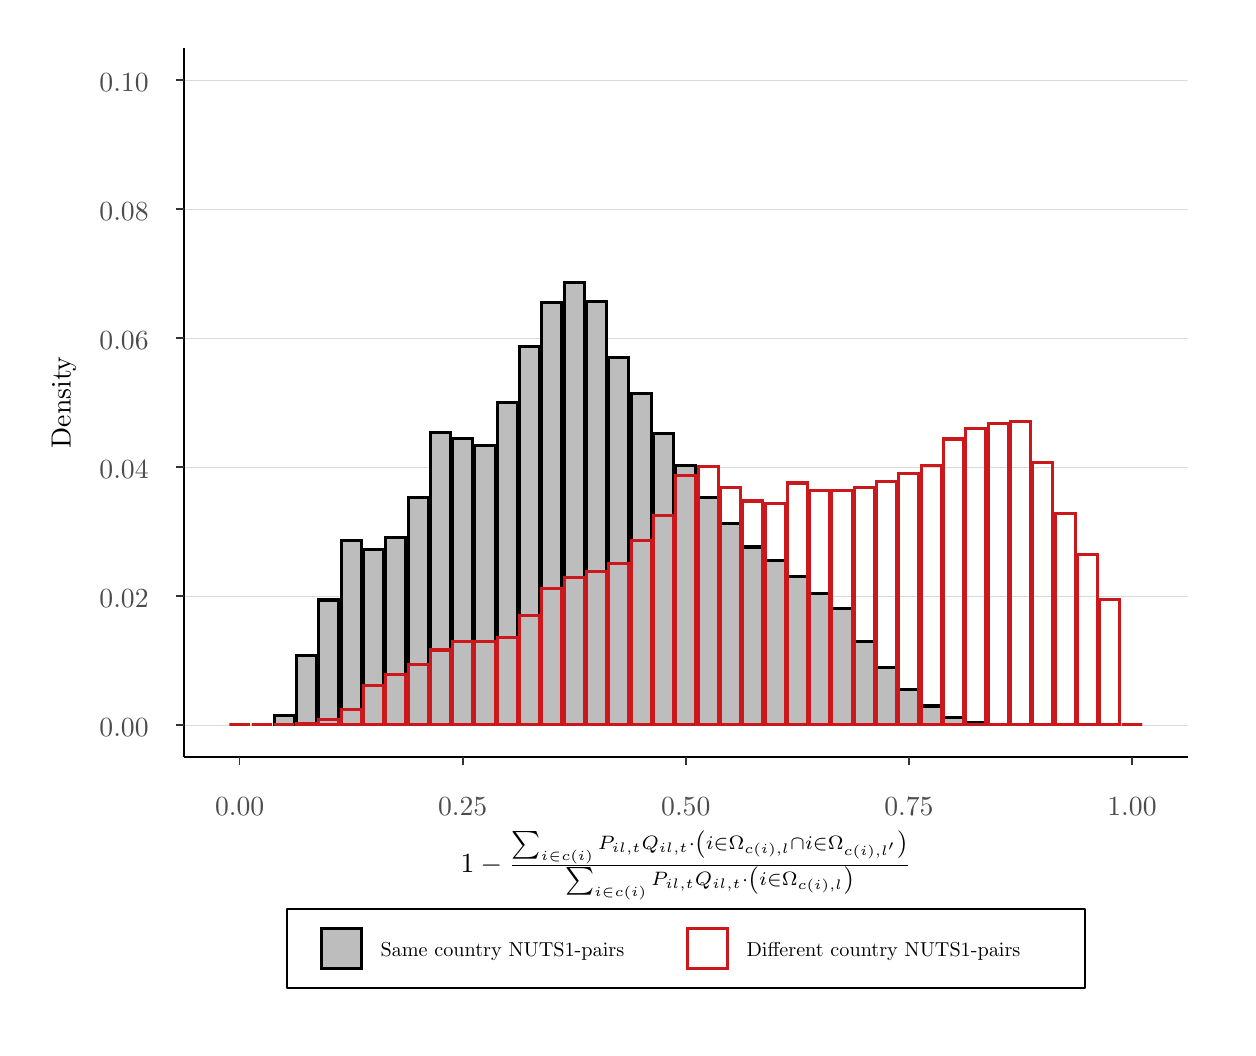
\begin{tikzpicture}[x=1pt,y=1pt]
\definecolor{fillColor}{RGB}{255,255,255}
\path[use as bounding box,fill=fillColor,fill opacity=0.00] (0,0) rectangle (433.62,361.35);
\begin{scope}
\path[clip] (  0.00,  0.00) rectangle (433.62,361.35);
\definecolor{drawColor}{RGB}{255,255,255}
\definecolor{fillColor}{RGB}{255,255,255}

\path[draw=drawColor,line width= 0.6pt,line join=round,line cap=round,fill=fillColor] ( -0.00,  0.00) rectangle (433.62,361.35);
\end{scope}
\begin{scope}
\path[clip] ( 56.47, 97.75) rectangle (419.17,354.12);
\definecolor{drawColor}{RGB}{255,255,255}

\path[draw=drawColor,line width= 0.3pt,line join=round] ( 56.47,132.71) --
	(419.17,132.71);

\path[draw=drawColor,line width= 0.3pt,line join=round] ( 56.47,179.32) --
	(419.17,179.32);

\path[draw=drawColor,line width= 0.3pt,line join=round] ( 56.47,225.94) --
	(419.17,225.94);

\path[draw=drawColor,line width= 0.3pt,line join=round] ( 56.47,272.55) --
	(419.17,272.55);

\path[draw=drawColor,line width= 0.3pt,line join=round] ( 56.47,319.16) --
	(419.17,319.16);

\path[draw=drawColor,line width= 0.3pt,line join=round] (116.89, 97.75) --
	(116.89,354.12);

\path[draw=drawColor,line width= 0.3pt,line join=round] (197.51, 97.75) --
	(197.51,354.12);

\path[draw=drawColor,line width= 0.3pt,line join=round] (278.12, 97.75) --
	(278.12,354.12);

\path[draw=drawColor,line width= 0.3pt,line join=round] (358.74, 97.75) --
	(358.74,354.12);
\definecolor{drawColor}{gray}{0.85}

\path[draw=drawColor,line width= 0.1pt,line join=round] ( 56.47,109.40) --
	(419.17,109.40);

\path[draw=drawColor,line width= 0.1pt,line join=round] ( 56.47,156.02) --
	(419.17,156.02);

\path[draw=drawColor,line width= 0.1pt,line join=round] ( 56.47,202.63) --
	(419.17,202.63);

\path[draw=drawColor,line width= 0.1pt,line join=round] ( 56.47,249.24) --
	(419.17,249.24);

\path[draw=drawColor,line width= 0.1pt,line join=round] ( 56.47,295.86) --
	(419.17,295.86);

\path[draw=drawColor,line width= 0.1pt,line join=round] ( 56.47,342.47) --
	(419.17,342.47);
\definecolor{drawColor}{RGB}{0,0,0}
\definecolor{fillColor}{gray}{0.74}

\path[draw=drawColor,line width= 1.1pt,line cap=rect,fill=fillColor] ( 72.95,109.40) rectangle ( 80.21,109.40);
\definecolor{drawColor}{RGB}{203,24,29}

\path[draw=drawColor,line width= 1.1pt,line cap=rect] ( 72.95,109.40) rectangle ( 80.21,109.40);
\definecolor{drawColor}{RGB}{0,0,0}

\path[draw=drawColor,line width= 1.1pt,line cap=rect,fill=fillColor] ( 81.01,109.40) rectangle ( 88.27,109.40);
\definecolor{drawColor}{RGB}{203,24,29}

\path[draw=drawColor,line width= 1.1pt,line cap=rect] ( 81.01,109.40) rectangle ( 88.27,109.40);
\definecolor{drawColor}{RGB}{0,0,0}

\path[draw=drawColor,line width= 1.1pt,line cap=rect,fill=fillColor] ( 89.08,109.40) rectangle ( 96.33,112.64);
\definecolor{drawColor}{RGB}{203,24,29}

\path[draw=drawColor,line width= 1.1pt,line cap=rect] ( 89.08,109.40) rectangle ( 96.33,109.40);
\definecolor{drawColor}{RGB}{0,0,0}

\path[draw=drawColor,line width= 1.1pt,line cap=rect,fill=fillColor] ( 97.14,109.40) rectangle (104.39,134.56);
\definecolor{drawColor}{RGB}{203,24,29}

\path[draw=drawColor,line width= 1.1pt,line cap=rect] ( 97.14,109.40) rectangle (104.39,109.79);
\definecolor{drawColor}{RGB}{0,0,0}

\path[draw=drawColor,line width= 1.1pt,line cap=rect,fill=fillColor] (105.20,109.40) rectangle (112.45,154.53);
\definecolor{drawColor}{RGB}{203,24,29}

\path[draw=drawColor,line width= 1.1pt,line cap=rect] (105.20,109.40) rectangle (112.45,111.43);
\definecolor{drawColor}{RGB}{0,0,0}

\path[draw=drawColor,line width= 1.1pt,line cap=rect,fill=fillColor] (113.26,109.40) rectangle (120.52,175.99);
\definecolor{drawColor}{RGB}{203,24,29}

\path[draw=drawColor,line width= 1.1pt,line cap=rect] (113.26,109.40) rectangle (120.52,115.09);
\definecolor{drawColor}{RGB}{0,0,0}

\path[draw=drawColor,line width= 1.1pt,line cap=rect,fill=fillColor] (121.32,109.40) rectangle (128.58,172.86);
\definecolor{drawColor}{RGB}{203,24,29}

\path[draw=drawColor,line width= 1.1pt,line cap=rect] (121.32,109.40) rectangle (128.58,123.62);
\definecolor{drawColor}{RGB}{0,0,0}

\path[draw=drawColor,line width= 1.1pt,line cap=rect,fill=fillColor] (129.38,109.40) rectangle (136.64,176.99);
\definecolor{drawColor}{RGB}{203,24,29}

\path[draw=drawColor,line width= 1.1pt,line cap=rect] (129.38,109.40) rectangle (136.64,127.51);
\definecolor{drawColor}{RGB}{0,0,0}

\path[draw=drawColor,line width= 1.1pt,line cap=rect,fill=fillColor] (137.45,109.40) rectangle (144.70,191.64);
\definecolor{drawColor}{RGB}{203,24,29}

\path[draw=drawColor,line width= 1.1pt,line cap=rect] (137.45,109.40) rectangle (144.70,131.10);
\definecolor{drawColor}{RGB}{0,0,0}

\path[draw=drawColor,line width= 1.1pt,line cap=rect,fill=fillColor] (145.51,109.40) rectangle (152.76,215.11);
\definecolor{drawColor}{RGB}{203,24,29}

\path[draw=drawColor,line width= 1.1pt,line cap=rect] (145.51,109.40) rectangle (152.76,136.47);
\definecolor{drawColor}{RGB}{0,0,0}

\path[draw=drawColor,line width= 1.1pt,line cap=rect,fill=fillColor] (153.57,109.40) rectangle (160.83,212.92);
\definecolor{drawColor}{RGB}{203,24,29}

\path[draw=drawColor,line width= 1.1pt,line cap=rect] (153.57,109.40) rectangle (160.83,139.54);
\definecolor{drawColor}{RGB}{0,0,0}

\path[draw=drawColor,line width= 1.1pt,line cap=rect,fill=fillColor] (161.63,109.40) rectangle (168.89,210.49);
\definecolor{drawColor}{RGB}{203,24,29}

\path[draw=drawColor,line width= 1.1pt,line cap=rect] (161.63,109.40) rectangle (168.89,139.38);
\definecolor{drawColor}{RGB}{0,0,0}

\path[draw=drawColor,line width= 1.1pt,line cap=rect,fill=fillColor] (169.69,109.40) rectangle (176.95,225.87);
\definecolor{drawColor}{RGB}{203,24,29}

\path[draw=drawColor,line width= 1.1pt,line cap=rect] (169.69,109.40) rectangle (176.95,141.10);
\definecolor{drawColor}{RGB}{0,0,0}

\path[draw=drawColor,line width= 1.1pt,line cap=rect,fill=fillColor] (177.76,109.40) rectangle (185.01,246.04);
\definecolor{drawColor}{RGB}{203,24,29}

\path[draw=drawColor,line width= 1.1pt,line cap=rect] (177.76,109.40) rectangle (185.01,149.02);
\definecolor{drawColor}{RGB}{0,0,0}

\path[draw=drawColor,line width= 1.1pt,line cap=rect,fill=fillColor] (185.82,109.40) rectangle (193.07,261.97);
\definecolor{drawColor}{RGB}{203,24,29}

\path[draw=drawColor,line width= 1.1pt,line cap=rect] (185.82,109.40) rectangle (193.07,158.82);
\definecolor{drawColor}{RGB}{0,0,0}

\path[draw=drawColor,line width= 1.1pt,line cap=rect,fill=fillColor] (193.88,109.40) rectangle (201.13,269.32);
\definecolor{drawColor}{RGB}{203,24,29}

\path[draw=drawColor,line width= 1.1pt,line cap=rect] (193.88,109.40) rectangle (201.13,162.57);
\definecolor{drawColor}{RGB}{0,0,0}

\path[draw=drawColor,line width= 1.1pt,line cap=rect,fill=fillColor] (201.94,109.40) rectangle (209.20,262.43);
\definecolor{drawColor}{RGB}{203,24,29}

\path[draw=drawColor,line width= 1.1pt,line cap=rect] (201.94,109.40) rectangle (209.20,164.89);
\definecolor{drawColor}{RGB}{0,0,0}

\path[draw=drawColor,line width= 1.1pt,line cap=rect,fill=fillColor] (210.00,109.40) rectangle (217.26,242.09);
\definecolor{drawColor}{RGB}{203,24,29}

\path[draw=drawColor,line width= 1.1pt,line cap=rect] (210.00,109.40) rectangle (217.26,167.82);
\definecolor{drawColor}{RGB}{0,0,0}

\path[draw=drawColor,line width= 1.1pt,line cap=rect,fill=fillColor] (218.06,109.40) rectangle (225.32,229.32);
\definecolor{drawColor}{RGB}{203,24,29}

\path[draw=drawColor,line width= 1.1pt,line cap=rect] (218.06,109.40) rectangle (225.32,175.99);
\definecolor{drawColor}{RGB}{0,0,0}

\path[draw=drawColor,line width= 1.1pt,line cap=rect,fill=fillColor] (226.13,109.40) rectangle (233.38,214.85);
\definecolor{drawColor}{RGB}{203,24,29}

\path[draw=drawColor,line width= 1.1pt,line cap=rect] (226.13,109.40) rectangle (233.38,184.92);
\definecolor{drawColor}{RGB}{0,0,0}

\path[draw=drawColor,line width= 1.1pt,line cap=rect,fill=fillColor] (234.19,109.40) rectangle (241.44,203.31);
\definecolor{drawColor}{RGB}{203,24,29}

\path[draw=drawColor,line width= 1.1pt,line cap=rect] (234.19,109.40) rectangle (241.44,199.41);
\definecolor{drawColor}{RGB}{0,0,0}

\path[draw=drawColor,line width= 1.1pt,line cap=rect,fill=fillColor] (242.25,109.40) rectangle (249.51,191.49);
\definecolor{drawColor}{RGB}{203,24,29}

\path[draw=drawColor,line width= 1.1pt,line cap=rect] (242.25,109.40) rectangle (249.51,202.80);
\definecolor{drawColor}{RGB}{0,0,0}

\path[draw=drawColor,line width= 1.1pt,line cap=rect,fill=fillColor] (250.31,109.40) rectangle (257.57,182.26);
\definecolor{drawColor}{RGB}{203,24,29}

\path[draw=drawColor,line width= 1.1pt,line cap=rect] (250.31,109.40) rectangle (257.57,195.36);
\definecolor{drawColor}{RGB}{0,0,0}

\path[draw=drawColor,line width= 1.1pt,line cap=rect,fill=fillColor] (258.37,109.40) rectangle (265.63,173.69);
\definecolor{drawColor}{RGB}{203,24,29}

\path[draw=drawColor,line width= 1.1pt,line cap=rect] (258.37,109.40) rectangle (265.63,190.31);
\definecolor{drawColor}{RGB}{0,0,0}

\path[draw=drawColor,line width= 1.1pt,line cap=rect,fill=fillColor] (266.44,109.40) rectangle (273.69,168.68);
\definecolor{drawColor}{RGB}{203,24,29}

\path[draw=drawColor,line width= 1.1pt,line cap=rect] (266.44,109.40) rectangle (273.69,189.45);
\definecolor{drawColor}{RGB}{0,0,0}

\path[draw=drawColor,line width= 1.1pt,line cap=rect,fill=fillColor] (274.50,109.40) rectangle (281.75,163.14);
\definecolor{drawColor}{RGB}{203,24,29}

\path[draw=drawColor,line width= 1.1pt,line cap=rect] (274.50,109.40) rectangle (281.75,196.81);
\definecolor{drawColor}{RGB}{0,0,0}

\path[draw=drawColor,line width= 1.1pt,line cap=rect,fill=fillColor] (282.56,109.40) rectangle (289.81,156.91);
\definecolor{drawColor}{RGB}{203,24,29}

\path[draw=drawColor,line width= 1.1pt,line cap=rect] (282.56,109.40) rectangle (289.81,193.98);
\definecolor{drawColor}{RGB}{0,0,0}

\path[draw=drawColor,line width= 1.1pt,line cap=rect,fill=fillColor] (290.62,109.40) rectangle (297.88,151.46);
\definecolor{drawColor}{RGB}{203,24,29}

\path[draw=drawColor,line width= 1.1pt,line cap=rect] (290.62,109.40) rectangle (297.88,194.02);
\definecolor{drawColor}{RGB}{0,0,0}

\path[draw=drawColor,line width= 1.1pt,line cap=rect,fill=fillColor] (298.68,109.40) rectangle (305.94,139.46);
\definecolor{drawColor}{RGB}{203,24,29}

\path[draw=drawColor,line width= 1.1pt,line cap=rect] (298.68,109.40) rectangle (305.94,195.19);
\definecolor{drawColor}{RGB}{0,0,0}

\path[draw=drawColor,line width= 1.1pt,line cap=rect,fill=fillColor] (306.74,109.40) rectangle (314.00,130.03);
\definecolor{drawColor}{RGB}{203,24,29}

\path[draw=drawColor,line width= 1.1pt,line cap=rect] (306.74,109.40) rectangle (314.00,197.41);
\definecolor{drawColor}{RGB}{0,0,0}

\path[draw=drawColor,line width= 1.1pt,line cap=rect,fill=fillColor] (314.81,109.40) rectangle (322.06,122.33);
\definecolor{drawColor}{RGB}{203,24,29}

\path[draw=drawColor,line width= 1.1pt,line cap=rect] (314.81,109.40) rectangle (322.06,200.16);
\definecolor{drawColor}{RGB}{0,0,0}

\path[draw=drawColor,line width= 1.1pt,line cap=rect,fill=fillColor] (322.87,109.40) rectangle (330.12,116.23);
\definecolor{drawColor}{RGB}{203,24,29}

\path[draw=drawColor,line width= 1.1pt,line cap=rect] (322.87,109.40) rectangle (330.12,202.99);
\definecolor{drawColor}{RGB}{0,0,0}

\path[draw=drawColor,line width= 1.1pt,line cap=rect,fill=fillColor] (330.93,109.40) rectangle (338.19,112.13);
\definecolor{drawColor}{RGB}{203,24,29}

\path[draw=drawColor,line width= 1.1pt,line cap=rect] (330.93,109.40) rectangle (338.19,212.72);
\definecolor{drawColor}{RGB}{0,0,0}

\path[draw=drawColor,line width= 1.1pt,line cap=rect,fill=fillColor] (338.99,109.40) rectangle (346.25,110.11);
\definecolor{drawColor}{RGB}{203,24,29}

\path[draw=drawColor,line width= 1.1pt,line cap=rect] (338.99,109.40) rectangle (346.25,216.49);
\definecolor{drawColor}{RGB}{0,0,0}

\path[draw=drawColor,line width= 1.1pt,line cap=rect,fill=fillColor] (347.05,109.40) rectangle (354.31,109.64);
\definecolor{drawColor}{RGB}{203,24,29}

\path[draw=drawColor,line width= 1.1pt,line cap=rect] (347.05,109.40) rectangle (354.31,218.21);
\definecolor{drawColor}{RGB}{0,0,0}

\path[draw=drawColor,line width= 1.1pt,line cap=rect,fill=fillColor] (355.12,109.40) rectangle (362.37,109.47);
\definecolor{drawColor}{RGB}{203,24,29}

\path[draw=drawColor,line width= 1.1pt,line cap=rect] (355.12,109.40) rectangle (362.37,219.05);
\definecolor{drawColor}{RGB}{0,0,0}

\path[draw=drawColor,line width= 1.1pt,line cap=rect,fill=fillColor] (363.18,109.40) rectangle (370.43,109.59);
\definecolor{drawColor}{RGB}{203,24,29}

\path[draw=drawColor,line width= 1.1pt,line cap=rect] (363.18,109.40) rectangle (370.43,204.07);
\definecolor{drawColor}{RGB}{0,0,0}

\path[draw=drawColor,line width= 1.1pt,line cap=rect,fill=fillColor] (371.24,109.40) rectangle (378.49,109.41);
\definecolor{drawColor}{RGB}{203,24,29}

\path[draw=drawColor,line width= 1.1pt,line cap=rect] (371.24,109.40) rectangle (378.49,185.65);
\definecolor{drawColor}{RGB}{0,0,0}

\path[draw=drawColor,line width= 1.1pt,line cap=rect,fill=fillColor] (379.30,109.40) rectangle (386.56,109.58);
\definecolor{drawColor}{RGB}{203,24,29}

\path[draw=drawColor,line width= 1.1pt,line cap=rect] (379.30,109.40) rectangle (386.56,170.82);
\definecolor{drawColor}{RGB}{0,0,0}

\path[draw=drawColor,line width= 1.1pt,line cap=rect,fill=fillColor] (387.36,109.40) rectangle (394.62,109.40);
\definecolor{drawColor}{RGB}{203,24,29}

\path[draw=drawColor,line width= 1.1pt,line cap=rect] (387.36,109.40) rectangle (394.62,154.58);
\definecolor{drawColor}{RGB}{0,0,0}

\path[draw=drawColor,line width= 1.1pt,line cap=rect,fill=fillColor] (395.42,109.40) rectangle (402.68,109.40);
\definecolor{drawColor}{RGB}{203,24,29}

\path[draw=drawColor,line width= 1.1pt,line cap=rect] (395.42,109.40) rectangle (402.68,109.40);
\end{scope}
\begin{scope}
\path[clip] (  0.00,  0.00) rectangle (433.62,361.35);
\definecolor{drawColor}{RGB}{0,0,0}

\path[draw=drawColor,line width= 0.6pt,line join=round] ( 56.47, 97.75) --
	( 56.47,354.12);
\end{scope}
\begin{scope}
\path[clip] (  0.00,  0.00) rectangle (433.62,361.35);
\definecolor{drawColor}{gray}{0.30}

\node[text=drawColor,anchor=base east,inner sep=0pt, outer sep=0pt, scale=  1.00] at ( 43.72,105.27) {0.00};

\node[text=drawColor,anchor=base east,inner sep=0pt, outer sep=0pt, scale=  1.00] at ( 43.72,151.88) {0.02};

\node[text=drawColor,anchor=base east,inner sep=0pt, outer sep=0pt, scale=  1.00] at ( 43.72,198.50) {0.04};

\node[text=drawColor,anchor=base east,inner sep=0pt, outer sep=0pt, scale=  1.00] at ( 43.72,245.11) {0.06};

\node[text=drawColor,anchor=base east,inner sep=0pt, outer sep=0pt, scale=  1.00] at ( 43.72,291.72) {0.08};

\node[text=drawColor,anchor=base east,inner sep=0pt, outer sep=0pt, scale=  1.00] at ( 43.72,338.34) {0.10};
\end{scope}
\begin{scope}
\path[clip] (  0.00,  0.00) rectangle (433.62,361.35);
\definecolor{drawColor}{gray}{0.20}

\path[draw=drawColor,line width= 0.6pt,line join=round] ( 53.72,109.40) --
	( 56.47,109.40);

\path[draw=drawColor,line width= 0.6pt,line join=round] ( 53.72,156.02) --
	( 56.47,156.02);

\path[draw=drawColor,line width= 0.6pt,line join=round] ( 53.72,202.63) --
	( 56.47,202.63);

\path[draw=drawColor,line width= 0.6pt,line join=round] ( 53.72,249.24) --
	( 56.47,249.24);

\path[draw=drawColor,line width= 0.6pt,line join=round] ( 53.72,295.86) --
	( 56.47,295.86);

\path[draw=drawColor,line width= 0.6pt,line join=round] ( 53.72,342.47) --
	( 56.47,342.47);
\end{scope}
\begin{scope}
\path[clip] (  0.00,  0.00) rectangle (433.62,361.35);
\definecolor{drawColor}{RGB}{0,0,0}

\path[draw=drawColor,line width= 0.6pt,line join=round] ( 56.47, 97.75) --
	(419.17, 97.75);
\end{scope}
\begin{scope}
\path[clip] (  0.00,  0.00) rectangle (433.62,361.35);
\definecolor{drawColor}{gray}{0.20}

\path[draw=drawColor,line width= 0.6pt,line join=round] ( 76.58, 95.00) --
	( 76.58, 97.75);

\path[draw=drawColor,line width= 0.6pt,line join=round] (157.20, 95.00) --
	(157.20, 97.75);

\path[draw=drawColor,line width= 0.6pt,line join=round] (237.82, 95.00) --
	(237.82, 97.75);

\path[draw=drawColor,line width= 0.6pt,line join=round] (318.43, 95.00) --
	(318.43, 97.75);

\path[draw=drawColor,line width= 0.6pt,line join=round] (399.05, 95.00) --
	(399.05, 97.75);
\end{scope}
\begin{scope}
\path[clip] (  0.00,  0.00) rectangle (433.62,361.35);
\definecolor{drawColor}{gray}{0.30}

\node[text=drawColor,anchor=base,inner sep=0pt, outer sep=0pt, scale=  1.00] at ( 76.58, 76.73) {0.00};

\node[text=drawColor,anchor=base,inner sep=0pt, outer sep=0pt, scale=  1.00] at (157.20, 76.73) {0.25};

\node[text=drawColor,anchor=base,inner sep=0pt, outer sep=0pt, scale=  1.00] at (237.82, 76.73) {0.50};

\node[text=drawColor,anchor=base,inner sep=0pt, outer sep=0pt, scale=  1.00] at (318.43, 76.73) {0.75};

\node[text=drawColor,anchor=base,inner sep=0pt, outer sep=0pt, scale=  1.00] at (399.05, 76.73) {1.00};
\end{scope}
\begin{scope}
\path[clip] (  0.00,  0.00) rectangle (433.62,361.35);
\definecolor{drawColor}{RGB}{0,0,0}

\node[text=drawColor,anchor=base,inner sep=0pt, outer sep=0pt, scale=  1.00] at (237.82, 56.13) {$1-\frac{\sum_{i \in c(i)}P_{il,t}Q_{il,t} \cdot \left(i \in \Omega_{c(i),l} \cap i \in \Omega_{c(i),l'} \right)}{\sum_{i \in c(i)} P_{il,t}Q_{il,t} \cdot \left(i \in \Omega_{c(i),l}\right)}$};
\end{scope}
\begin{scope}
\path[clip] (  0.00,  0.00) rectangle (433.62,361.35);
\definecolor{drawColor}{RGB}{0,0,0}

\node[text=drawColor,rotate= 90.00,anchor=base,inner sep=0pt, outer sep=0pt, scale=  1.00] at ( 15.49,225.94) {Density};
\end{scope}
\begin{scope}
\path[clip] (  0.00,  0.00) rectangle (433.62,361.35);
\definecolor{drawColor}{RGB}{0,0,0}
\definecolor{fillColor}{RGB}{255,255,255}

\path[draw=drawColor,line width= 0.6pt,line join=round,line cap=round,fill=fillColor] ( 93.65, 14.45) rectangle (381.98, 42.80);
\end{scope}
\begin{scope}
\path[clip] (  0.00,  0.00) rectangle (433.62,361.35);

\path[] (104.65, 19.95) rectangle (122.00, 37.30);
\end{scope}
\begin{scope}
\path[clip] (  0.00,  0.00) rectangle (433.62,361.35);
\definecolor{drawColor}{RGB}{0,0,0}
\definecolor{fillColor}{gray}{0.74}

\path[draw=drawColor,line width= 1.1pt,line cap=rect,fill=fillColor] (106.08, 21.38) rectangle (120.58, 35.88);
\end{scope}
\begin{scope}
\path[clip] (  0.00,  0.00) rectangle (433.62,361.35);

\path[] (236.91, 19.95) rectangle (254.26, 37.30);
\end{scope}
\begin{scope}
\path[clip] (  0.00,  0.00) rectangle (433.62,361.35);
\definecolor{drawColor}{RGB}{203,24,29}

\path[draw=drawColor,line width= 1.1pt,line cap=rect] (238.34, 21.38) rectangle (252.84, 35.88);
\end{scope}
\begin{scope}
\path[clip] (  0.00,  0.00) rectangle (433.62,361.35);
\definecolor{drawColor}{RGB}{0,0,0}

\node[text=drawColor,anchor=base west,inner sep=0pt, outer sep=0pt, scale=  0.73] at (127.50, 25.60) {Same country NUTS1-pairs};
\end{scope}
\begin{scope}
\path[clip] (  0.00,  0.00) rectangle (433.62,361.35);
\definecolor{drawColor}{RGB}{0,0,0}

\node[text=drawColor,anchor=base west,inner sep=0pt, outer sep=0pt, scale=  0.73] at (259.76, 25.60) {Different country NUTS1-pairs};
\end{scope}
\end{tikzpicture}
